\documentclass[11pt, twoside]{article}

% Erlaube einfaches copy & paste aus der generierten pdf
\usepackage[T1]{fontenc}
\usepackage[utf8]{inputenc}

% Deutsche Bezeichnungen wie etwa "Inhaltsverzeichnis", statt "Contents"
\usepackage[german]{babel}

% Deutsche Absätze
\parindent 0pt

% Dieses Package ermöglich einfügen von Bildern mittels \includegraphics
\usepackage{graphicx}

% Zwinge Latex zum einfügen von bildern dort wo man sie im tex 
% Dokument hinterlegt mittels \begin{figure}[H]   
\usepackage{float}

% Syntax Highlighting 
\usepackage{minted}

\usepackage[autostyle,german=quotes]{csquotes}

% Für Hintergrundbilder mittels \AddToShipoutPicture
\usepackage{eso-pic}

% Bilder transparent machen
\usepackage{transparent}

% Fallunterscheidungen wie etwa gerade und ungerade Seiten
\usepackage{ifthen}

% Einfügen von Tabellen
\usepackage{tabularx}

% Literaturverzeichnisse verwenden
% backref=true - referenziert von Literaturverzeichnis zurück auf die Seite wo zitiert wurde
\usepackage[style=authortitle, natbib, backend=biber, backref=true]{biblatex}
% Nummer der Zitation nicht hochgestellt, sondern sondern mit
% normaler Textgröße und einem Punkt nach der Nummer
% Beispiel: 1. Teller,”Visibility computations in densely occluded polyhedral environments.“, S. 19
\makeatletter% 
\long\def\@makefntext#1{% 
  \parindent 1em\noindent \hb@xt@ 1.8em{\hss  \hbox {{\normalfont \@thefnmark }}. }#1}%
\makeatother

% Texte für die zurückreferenzierung definieren
\DefineBibliographyStrings{german}{%
  backrefpage = {Zitiert auf der Seite},% originally "cited on page"
  backrefpages = {Zitiert auf den Seiten},% originally "cited on pages"
}

% Links mit Sprungmarken
\usepackage{hyperref}
\hypersetup{
  colorlinks=true,
  linkcolor=black, % Setz die Farbe von Links im 
                   % Inhaltsverzeichnis zurück auf schwarz
  citecolor=black, % Farbe von Literaturlinks = schwarz
  urlcolor=blue    % Farbe von URLs = blau     
}


% Referezieren von Kapiteln mit ihrem Titel
\usepackage{nameref}

% Einfügen von PDFs
\usepackage{pdfpages} 

% Seitenränder
\usepackage{geometry}
\geometry{a4paper, top=20mm, left=40mm, right=20mm, bottom=20mm, headsep=12mm, footskip=12mm}

% Package zum hinzufügen eines Glossars
\usepackage{glossaries}  
\setacronymstyle{long-short}  
\newacronym{eler}{ELER}{Europäischer Landwirtschaftsfond für die Entwicklung des ländlichen Raum}  

% Auf gleiche footnote erneut verweisen mit cleveref
% Achtung: Wenn cleveref nicht zum ende geladen wird gibt es evtl. die Fehlermeldung: Package cleveref Error: cleveref must be loaded after amsmath!.
\usepackage{cleveref}
% Auf erneut verweisen
\crefformat{footnote}{#2\footnotemark[#1]#3}  

\addbibresource{literatur/literatur.bib}

\begin{document}
 

\begin{center}
    

    %\includegraphics[width=0.5\paperwidth]{img/logo/hs_harz_logo.png}

    \vspace{20mm}

    \Huge
    \textsc{Flutter vs Complexity}

    \vspace{5mm}

    \Large
    \textsc{Eine Eallstudie zur Lösung einer komplexen Problemstellung mit Hilfe einer Reihe an Softwaretechnischer Hilfsmittel mit Flutter}
    \vfill
    
    % https://pascalhertleif.de/artikel/richtlinien-fur-fallstudien-in-der-software-entwicklung/

    \normalsize
    Vorgelegt von:

    \textbf{Alexander Johr}

    Meine Adresse

    \vspace{20mm}

    \begin{tabular}{r c}
        Erstprüfer: & Prof. Jürgen Singer Ph.D. \\
        Zweitprüfer: & Prof. Daniel Ackermann \\
        Datum: & 02.11.2020 \\
    \end{tabular}

    \vspace{5mm}

\end{center}


  
\newpage\null\thispagestyle{empty}\newpage

\newpage
\thispagestyle{empty}

Hochschule Harz\newline
Fachbereich Automatisierung und Informatik
\vfill
\begin{center}

\large{\textsc{Thema und Aufgabenstellung der Masterarbeit}}


\large{\textsc{MA AI ??/2021}}

\vfill

\large{\textsc{für Herrn Alexander Johr}}

\vfill

%\vfill

\large{\textsc{Entwicklung einer Formularanwendung mit Kompatibilitätsvalidierung der Einfach- und Mehrfachauswahl-Eingabefelder}}



\end{center}

\vfill

%gut darlegen könnendie methode spielt mehr die rolle


%andeuten nicht ins detail

%ich möchte mich testing


%kern des themas

%immer zurück kommen

%höhere eigen zum ergebis

%das liebesleben der tennisbällen unter einfluss des mondscheins

%größtmögliche unfall der passiert mal wahrscheinlichkeit 

%kompliziertheit komplexität

%werner von braun
%triebwerke geschrottet

%doku 
%arte 3 sat
%allgemein menschheit in den weltraum

%feindifferenziert


%Frage an Herr Ackermann / Singer: Vergleich mit Angular Dart, Angular allgemein, XAML WPF, evtl. etwas 

%Aber nicht alle

%Deshalb Fallstudie, richtig?



Das Thünen-Institut für Ländliche Räume erhebt Daten von Maßnahmen
 des Europäischen
Landwirtschaftsfonds für die Entwicklung des ländlichen Raums
 (ELER).
Um die Eingabe für die Wissenschaftler des Instituts zu beschleunigen
 und um fehlerhafte Eingaben zu minimieren, soll eine 
 spezielle Formularanwendung entwickelt werden.
Neben herkömmlichen Freitextfeldern beinhaltet das gewünschte Formular zum Großteil Eingabefelder für Einfach- und Mehrfachauswahl.
Je nach Feld kann die Anzahl der Auswahloptionen mitunter zahlreich sein.
Dem Nutzer sollen daher nur solche Auswahloptionen angeboten werden,
die zusammen mit der zuvor getroffenen Auswahl sinnvoll sind.

\vspace{14pt}

Im Wesentlichen ergibt sich die Kompatibilität 
der Auswahloptionen aus der Bedingung, 
dass für dasselbe oder ein anderes Eingabefeld eine Auswahlmöglichkeit gewählt bzw.
nicht gewählt ist. Diese Bedingungen müssen durch 
Konjunktion und Disjunktion verknüpft werden können.
In Sonderfällen muss ein Formularfeld jedoch auch 
die Konfiguration einer vom Standard abweichenden Bedingung
ermöglichen. 
Wird dennoch versucht,
eine deaktivierte Option zu selektieren, wäre eine Anzeige der
inkompatiblen sowie der stattdessen notwendigen Auswahl ideal.

\vspace{14pt}
Die primäre Zielplattform der Anwendung ist das Desktop-Betriebssystem
Microsoft Windows 10.
Idealerweise ist die Formularanwendung auch auf weiteren Desktop-Plattformen sowie
mobilen Endgeräten wie Android- und iOS-Smartphones und -Tablets
lauffähig. Die Serialisierung der eingegebenen Daten genügt dem Institut 
zunächst als Ablage einer lokalen Datei im JSON-Format. 
%Nach der Testphase des Eingabeformulars erfolgt der Import der Daten in das Relationale Datenbank-Management System ProstgreSQL. 

% Beim Versuch, eine inkompatible Auswahl zu selektieren,
% könnte die Visualisierung eines Mengendiagramms der erforderlichen und invaliden
% Auswahlfelder und die User Experience weiter verbessern.
% Als Ergebnis der Anforderungsanalyse wurde 
% ein UI-Framework ausgewählt,
% welches neben weiteren Auswahlkriterien 
% insbesondere ein hohes Maß an Flexibilität erlaubt: Flutter.





%Die freiheiten in der Oberflächenentwicklung 


%Ziel dieser Masterarbeit ist die Entwicklung der Formular-Anwendung 
%und dabei den Entwicklungsschitteprozess und die 

%Flutter bietet arbeitet mit funktionaler UI. Damit gibt Flutter die Wahl des Zustandsmanagements.


%Dies bietet einige Vorlteile. Koontrolle über die Performance.
%Vereinfachte Fehlersuche in der UI. Freiheiten in der Entwicklung der UI.
%Konfiguration von wiederverwendbaren Oberflächenkomponenten mithilfe des Strategy Entwurfsmusters.
%Doch es ergeben sich auch Nachteile: 
%Es gibt keine goto Methode für zustandsmanagement sondern eine Auswahl der 
%richtigen Methoe muss auf Grundlage der Anfforderungen gewählt werden.

%Zier der Arbeit ist es die Vorteile und Nachteile näher zubeleuchten.
%Dies soll mit der Entwicklung einer Anwendung in Flutter begleitet werden. Die Anwendung soll eine komplexes Eingabe-Formular für das Thünen institut in Braunschweig sein.



%Templates <-> Functional UI

%Exceptions <-> Hot Reload

%Stragety Pattern

%Reguläre ausdrücke

%Refactoring

%Programmgenerierung JSON AOT vs C\# Reflection


%Kontrolle

%Nachteile

%Provider BloC <-> Provider
%Eine  Data Binding

%Die zwei b Die beiden 

%Performance

%Die Produkte QlikView und Qlik Sense - Business Intelligence Software des Software\-unter\-nehmens Qlik - bieten ihren Anwendern mit einer Reihe an unterschiedlichen Diagramm\-typen einen Überblick über ihre Geschäftsdaten mittels Ad-hoc-Analysen. Nicht alle Wünsche der Anwender lassen sich über die Konfigurations\-möglich\-keiten dieser vorgefertigten Diagramme abdecken. Eine Alternative stellen die sogenannten Extension Objects und Document Extensions dar, die mit mithilfe von Webtechnologien wie JavaScript, HTML, CSS und XML entwickelt werden können. Die Entwicklung von Programmen mit JavaScript erweist sich jedoch gegenüber der Entwicklung mit anderen Programmiersprachen als sehr mühsam.


%Ziel dieser Bachelorarbeit ist es die Entwicklung dieser Extension Objects sowie Document Extensions mit der Programmiersprache Dart von Google umzusetzen, da sich diese für die Entwicklung skalierbarer und strukturierter Webanwendungen eignet. Die Arbeit bietet einen Leitfaden wie solche Extensions mit Dart entwickelt werden können und welche Vor- und Nachteile dies gegenüber der Entwicklung mit JavaScript bietet. 


%Die Bachelorarbeit beinhaltet folgende Teilaufgaben:
%\begin{itemize}
%	\itemsep0em
%	\item Analyse der Unterschiede von QlikView 11 und Qlik Sense bei der Entwicklung von Extension Objects sowie von Document Extensions
%	\item Analyse der Einschränkungen von Extensions Objects gegenüber der von QlikView 11 und Qlik Sense mitgelieferten Sheet Objects
%	\item Analyse der Auswirkungen der Extensions auf die Performance
%	\item Analyse der Vor- und Nachteile der Entwicklung von Extensions mit Dart im Vergleich zur Entwicklung von Extensions mit JavaScript
%	\item Entwicklung von zeitsparenden Methoden zur Entwicklung von Extensions
%	\item Bewertung der Ergebnisse
%\end{itemize}

\vspace{14pt}
Die Masterarbeit umfasst folgende Teilaufgaben:
\begin{itemize}
    \itemsep0em
\item Analyse der Anforderungen an die Formularanwendung
\item Evaluation der angemessenen Technologie für die Implementierung
\item Entwurf und Umsetzung der Übersichts- und Eingabeoberfläche
\item Konzeption und Implementierung der Validierung der Eingabefelder
\item Entwicklung von automatisierten Testfällen zur Qualitätskontrolle
\item Bewertung der Implementierung und Vergleich mit den Wunschkriterien
\end{itemize}


%Die Freiheiten der Oberflächenentwicklung in Flutter sollen genutzt werden, um 
%visuellen Komponenten zu erstellen, die durch Einsatz des Strategie-Entwurfsmusters
%im hohen Maße anpassbar sind.



%Da die Aktualisierung von Flutter-Views nicht automatisch erfolgt, muss ein angemessenes 
%Zustandsmanagement evaluiert und eingesetzt werden.
%Eine angemessene Technologie zur Serialisierung soll gewählt und 
%das Persistieren der eingegebenen Datensätze damit umgesetzt werden.
%Durch die Menge der Auswahlfelder ist bei Weiterentwicklung der APIs mit 
%hohem Migrationsaufwand der Codebasis zu rechnen. Der Einsatz von regulären Ausdrücken
%soll helfen, den Prozess zu automatisieren. Die Entwicklung automatisierter Testfälle
%soll weiterhin ermöglichen, Fehler bei der Weiterentwicklung zeitnah zu erkennen.



%Die Masterarbeit beinhaltet damit folgende Teilaufgaben:
%\begin{itemize}
%	\itemsep0em
%	\item Evaluation des Zustandsmanagements und Implementierung des View Models
%    \item Entwicklung von wiederverwendbarer Komponenten des Views und Anpassung dieser mit dem Strategie Entwurfsmuster
%    \item Auswahl der Technologie zur Serialisierung und Implementierung der Persistierung des Models
%	\item Migration der Codebasis auf aktualisierte APIs mittels Regulärer Ausdrücke
%	\item Entwicklung von Automatisierten Testfällen
%\end{itemize}

\vfill
\vfill

\begin{tabularx}{\textwidth}{@{} *2{>{\centering\arraybackslash}X}@{}}
Prof. Jürgen Singer Ph.D. & Prof. Daniel Ackermann \\
1. Prüfer                 & 2. Prüfer	 \\
\end{tabularx}	        


\include{misc/Inhaltsverzeichnis}
\include{misc/Abbildungsverzeichnis.tex} 
%List of Listings umbenennen
\renewcommand{\listoflistingscaption}{Listingsverzeichnis}

%Listingsverzeichnis
\addcontentsline{toc}{section}{Listingsverzeichnis}
\listoflistings


\setlength{\parskip}{14pt}

\section{Technologie Auswahl}

Dieses Kapitel behandelt die Auswahl der Frontend-Technologie für die Umsetzung der Formular-Anwendung. Dazu  werden im ersten Schritt die dafür in Frage kommende Technologien identifiziert.  Anschließend wird der Trend der Popularität dieser Technologien miteinander verglichen. Die daraus resultierenden Kandidaten sollen dann einem detaillierter untersucht werden. In Hinblick auf die Anforderungen an die Formular-Anwendung soll dabei die angemessenste Frontend-Technologie ausgewählt werden.

\subsection{Trendanalyse}

Zwei Quellen wurden für die Analyse der Technologie-Trends ausgewählt: die Ergebnisse der jährlichen Stack Overflow Umfragen und das Such-Interesse von Google Trends. 

\paragraph{Stack Overflow Umfrage}
Die Internet-Plattform Stack Overflow richtet sich an Softwareentwickler und bietet ihren Nutzern die Möglichkeiten, Fragen zu stellen, Antworten einzustellen und Antworten anderer Nutzer auf- und abzuwerten. 
Besonders für Fehlermeldungen, die häufig während der Softwareentwicklung auftreten, findet man auf dieser Plattform rasch die Erklärung und den Lösungsvorschlag gleich mit. Dadurch lässt sich auch die Herkunft des Domain-Namens herleiten:

\begin{quotation}
We named it Stack Overflow, after a common type of bug that causes software to crash -- plus, the domain name stackoverflow.com happened to be available. - Joel Spolsky, Mitgründer von Stack Overflow \footnote{\cite{TheUnprovenPath}}
\end{quotation}

Aufgrund des Erfolgsrezepts von Stack Overflow ist die Plattform kaum einem Softwareentwickler unbekannt. Dementsprechend nehmen auch jährlich tausende Entwickler an den von Stack Overflow herausgegebenen Umfragen teil. Seit  2013 beinhaltet die Umfragen auch die Angabe der aktuell genutzten und in Zukunft gewünschten Frontend-Technologien.
Stackoverflow erstellt aus diesen gesammelten Daten Auswertungen und Übersichten. Doch gleichzeitig werden die zugrundeliegenden Daten veröffentlicht. \footnote{\cite{StackOverflowInsights}} 

Um den Trend der Beliebtheit der Frontend-Technologien aufzuzeigen, wurde ein Jupyter Notebook erstellt. Es transformiert die Daten in ein einheitliches Format, da die  Umfrageergebnisse von Jahr zu Jahr in einer unterschiedlichen Struktur abgelegt wurden. Anschließend erstellt es Diagramme, die im Folgenden analysiert werden. Das Jupyter Notebook ist im  Anhang zu finden.

\paragraph{Google Trends} Suchanfragen die an die Suchmaschine Google  abgesetzt werden, lassen sich  über den Dienst Google Trends  als Trenddiagramm Visualisieren. Um das relative Such-Interesse abzubilden werden die Ergebnisse normalisiert um die Ergebnisse auf einer Skala von 0 bis 100 Darstellen zu können. \footnote{Vgl. \cite{GoogleTrendsHilfe}}

\begin{quotation}
Google Trends ist keine wissenschaftliche Umfrage und sollte nicht mit Umfragedaten verwechselt werden. Es spiegelt lediglich das Suchinteresse an bestimmten Themen wider. \footnote{\cite{GoogleTrendsHilfe}}
\end{quotation}

Genau aus diesem Grund wird Google Trends im folgenden lediglich zum Abgleich der Ergebnisse der Stackoverflow Umfrage  eingesetzt.


\subsubsection{Eingestellte Projekte}



\subsubsection{Stack Overflow Umfrage}




\begin{figure}[htbp]
	\centering
    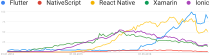
\includegraphics[width=1.0\textwidth]{images/charts/Google Trends/frameworks.pdf}
	\caption[ Weltweit Ein QlikView Sheet mit diversen Sheet Objects]{Ein QlikView Sheet mit diversen Sheet Objects, Quelle: Eigene Abbildung}
	\label{fig:Sheet1}
\end{figure}


\begin{figure}[htbp]
	\centering
    \includegraphics[width=1.0\textwidth]{images/charts/Google Trends/frameworks_plot.pdf}
	\caption[ Weltweit Ein QlikView Sheet mit diversen Sheet Objects]{Ein QlikView Sheet mit diversen Sheet Objects, Quelle: Eigene Abbildung}
	\label{fig:Sheet2}
\end{figure}


\begin{appendix} 

  %\renewcommand\section{\stdsection}
  
  \newpage
  
  \section*{Anhang} 
  \addcontentsline{toc}{section}{Anhang}%\addtocontents{toc}{\vfill}
  \renewcommand{\thesubsection}{\Alph{subsection}}
  
  \subsection{Quelltexte} 
  \label{lab:ScreenshotsVonQlikView}
  

\begin{listing}[H]
	\label{lst:quelltext1}

    \begin{minted}[
        linenos, % Quelltextzeilen anzeigen
        numbersep=5pt, %Abstand
        firstnumber=1,
        frame=lines,
        fontsize=\small,
        framesep=2mm,
		tabsize=4,
		breaklines,
		breakafter=_@|
        ]{dart}
import 'package:flutter/material.dart';
import 'input.dart';

void main() => runApp(MyApp());

class MyApp extends StatelessWidget {
  @override
  Widget build(BuildContext context) => MaterialApp(
		home: Scaffold(
		  body: MyCustomForm(),
		),
	  );
}

final emailPattern = new RegExp(
    r'^(([^<>()\[\]\\.,;:\s@\enquote{]+(\.[^<>()\[\]\\.,;:\s@} ]+)*)|(\enquote{.+} ))@((\[[0-9]{1,3}\.[0-9]{1,3}\.[0-9]{1,3}\.[0-9]{1,3}\])|(([a-zA-Z\-0-9]+\.)+[a-zA-Z]{2,}))$');

class MyCustomForm extends StatefulWidget {
  @override
  MyCustomFormState createState() => MyCustomFormState();
}

class MyCustomFormState extends State<MyCustomForm> {
  final _formKey = GlobalKey<FormState>();

  @override
  Widget build(BuildContext context) => Form(
		key: _formKey,
		child: Padding(
		  padding: const EdgeInsets.all(8.0),
		  child: Column(
			children: [
			  Input(label: \enquote{Name} ),
			  Input(
				  label: \enquote{Email} ,
				  validator: (value) {
					if (value == null || !emailPattern.hasMatch(value)) {
					  return 'Invalid Email Format';
					}
					return null;
				  }),
			  Input(label: \enquote{Password} ),
			  Padding(
				padding: const EdgeInsets.symmetric(vertical: 16.0),
				child: ElevatedButton(
				  onPressed: () {
					if (_formKey.currentState!.validate()) {
					  ScaffoldMessenger.of(context).showSnackBar(
						  SnackBar(content: Text('Processing Data')));
					}
				  },
				  child: Text('Submit'),
				),
			  ),
			],
		  ),
		),
	  );
}
		
    \end{minted}

    \caption[main.dart]{main.dart Datei}
\end{listing}


\begin{listing}[H]
	\label{lst:quelltext2}

    \begin{minted}[
        linenos, % Quelltextzeilen anzeigen
        numbersep=5pt, %Abstand
        firstnumber=1,
        frame=lines,
        fontsize=\small,
        framesep=2mm,
		tabsize=4,
		breaklines,
		breakafter=_@|
        ]{javascript}
export default {
	name: {required: {value: true, message: 'Name is required'}},
	email: {
	  required: {value: true, message: 'Email is required'},
	  pattern: {
		value: /^(([^<>()\[\]\\.,;:\s@\enquote{]+(\.[^<>()\[\]\\.,;:\s@} ]+)*)|(\enquote{.+} ))@((\[[0-9]{1,3}\.[0-9]{1,3}\.[0-9]{1,3}\.[0-9]{1,3}\])|(([a-zA-Z\-0-9]+\.)+[a-zA-Z]{2,}))$/,
		message: 'Invalid Email Format',
	  },
	},
	password: {
	  required: {value: true, message: 'Password is required'},
	},
  };
    \end{minted}

    \caption[validation.tsx]{validation.tsx Datei}
\end{listing}


\begin{listing}[H]
	\label{lst:quelltext3}

    \begin{minted}[
        linenos, % Quelltextzeilen anzeigen
        numbersep=5pt, %Abstand
        firstnumber=1,
        frame=lines,
        fontsize=\small,
        framesep=2mm,
		tabsize=4,
		breaklines,
		breakafter=_@|
        ]{dart}
final emailPattern = new RegExp(
	r'^(([^<>()\[\]\\.,;:\s@\enquote{]+(\.[^<>()\[\]\\.,;:\s@} ]+)*)|(\enquote{.+} ))@((\[[0-9]{1,3}\.[0-9]{1,3}\.[0-9]{1,3}\.[0-9]{1,3}\])|(([a-zA-Z\-0-9]+\.)+[a-zA-Z]{2,}))$');

validateEmail(value) {
  if (value == null || !emailPattern.hasMatch(value))
	return 'Invalid Email Format';
  else
	return null;
}

validateNotEmpty(String label, value) {
  if (value == null || value.isEmpty)
	return '$label is required';
  else
	return null;
}		
    \end{minted}

    \caption[validation.dart]{validation.dart Datei}
\end{listing}


\begin{listing}[H]
	\label{lst:quelltext4}

    \begin{minted}[
        linenos, % Quelltextzeilen anzeigen
        numbersep=5pt, %Abstand
        firstnumber=1,
        frame=lines,
        fontsize=\small,
        framesep=2mm,
		tabsize=4,
		breaklines,
		breakafter=_@|
        ]{dart}
import 'package:example_form_app/validation.dart';
import 'package:flutter/material.dart';

class Input extends StatelessWidget {
  final String label;
  final FormFieldValidator<String>? validator;

  const Input({required this.label, this.validator});

  @override
  Widget build(BuildContext context) => TextFormField(
	  decoration: InputDecoration(labelText: label),
	  validator: validator ?? (value) => validateNotEmpty(label, value));
}
    \end{minted}

    \caption[input.dart]{input.dart Datei}
\end{listing}













\begin{listing}[H]
	\label{lst:quelltext5}

    \begin{minted}[
        linenos, % Quelltextzeilen anzeigen
        numbersep=5pt, %Abstand
        firstnumber=1,
        frame=lines,
        fontsize=\small,
        framesep=2mm,
		tabsize=4,
		breaklines,
		breakafter=_@|
        ]{javascript}
import * as React from 'react';
import { TextInput, KeyboardAvoidingView, findNodeHandle } from 'react-native';
import { ValidationOptions, FieldError } from 'react-hook-form';

interface ValidationMap {
  [key: string]: ValidationOptions;
}

interface ErrorMap {
  [key: string]: FieldError | undefined;
}

interface Props {
  children: JSX.Element | JSX.Element[];
  register: (
    field: { name: string },
    validation?: ValidationOptions
  ) => void;
  errors: ErrorMap;
  validation: ValidationMap;
  setValue: (name: string, value: string, validate?: boolean) => void;
}
\end{minted}


\caption[Form.tsx]{Form.tsx Datei}
\end{listing}

\begin{listing}[H]
	\label{lst:quelltext6}
    \inputminted[lastline=23, linenos, numbersep=5pt, firstnumber=1, frame=lines, fontsize=\small, framesep=2mm, tabsize=4, breaklines, breakafter=_@|]
    {typescript}
    {source_code/flutter_vs_react_native/react_native/example_form_app/form-in-react-native-the-right-way/components/Form.tsx}
\caption[Form.tsx]{Form.tsx Datei}
\end{listing}
 
\begin{listing}[H]
	\label{lst:quelltext7}
    \inputminted[firstline=24, linenos, numbersep=5pt, firstnumber=24, frame=lines, fontsize=\small, framesep=2mm, tabsize=4, breaklines, breakafter=_@|]
    {typescript}
    {source_code/flutter_vs_react_native/react_native/example_form_app/form-in-react-native-the-right-way/components/Form.tsx}
\caption[Form.tsx]{Form.tsx Datei}
\end{listing}




\begin{listing}[H]
	\label{lst:quelltext8}
    \begin{minted}[
        linenos, % Quelltextzeilen anzeigen
        numbersep=5pt, %Abstand
        firstnumber=1,
        frame=lines,
        fontsize=\small,
        framesep=2mm,
		tabsize=4,
		breaklines,
		breakafter=_@|
        ]{javascript}
import * as React from 'react';
import {
  View,
  TextInput,
  Text,
  StyleSheet,
  ViewStyle,
  TextStyle,
  TextInputProps,
} from 'react-native';
import { FieldError } from 'react-hook-form';
interface Props extends TextInputProps {
  name: string;
  label?: string;
  labelStyle?: TextStyle;
  error?: FieldError | undefined;
}

export default React.forwardRef<any, Props>(
  (props, ref): React.ReactElement => {
	const { label, labelStyle, error, ...inputProps } = props;

	return (
	  <View style={styles.container}>
		{label && <Text style={[styles.label, labelStyle]}>{label}</Text>}
		<TextInput
		  autoCapitalize=\enquote{none}
		  ref={ref}
		  style={[styles.input, { borderColor: error ? '#fc6d47' : '#c0cbd3' }]}
		  {...inputProps}
		/>
		<Text style={styles.textError}>{error && error.message}</Text>
	  </View>
	);
  }
);

const styles = StyleSheet.create({
  container: {
	marginVertical: 8,
  },
  input: {
	borderWidth: 1,
	paddingLeft: 5,
  },
  label: {
	paddingVertical: 5,
  },
  textError: {
	color: '#fc6d47',
  },
});	
\end{minted}


\caption[Input.tsx]{Input.tsx Datei}
\end{listing}


 

\begin{listing}[H]
	\label{lst:quelltext9}

    \begin{minted}[
        linenos, % Quelltextzeilen anzeigen
        numbersep=5pt, %Abstand
        firstnumber=1,
        frame=lines,
        fontsize=\small,
        framesep=2mm,
		tabsize=4,
		breaklines,
		breakafter=_@|
        ]{javascript}
import * as React from 'react';
import {
  Text,
  View,
  StyleSheet,
  Button,
  Alert,
  ScrollView,
} from 'react-native';

import { useForm } from 'react-hook-form';

import Input from './components/Input';
import Form from './components/Form';
import validation from './validation';

type FormData = {
  name: string;
  email: string;
  password: string;
};

export default () => {
  const { handleSubmit, register, setValue, errors } = useForm<FormData>();

  const onSubmit = (data: FormData) => {
	Alert.alert('data', JSON.stringify(data));
  };

  return (
	  <View style={styles.formContainer}>
		<Form {...{ register, setValue, validation, errors }}>
		  <Input name=\enquote{name} label=\enquote{Name } />
		  <Input name=\enquote{email} label=\enquote{Email} />
		  <Input name=\enquote{password} label=\enquote{Password} secureTextEntry={true} />
		  <Button title=\enquote{Submit} onPress={handleSubmit(onSubmit)} />
		</Form>
	  </View>
  );
};

const styles = StyleSheet.create({
  formContainer: {
	padding: 8,
	flex: 1,
  }
});		
\end{minted}


\caption[App.tsx]{App.tsx Datei}
\end{listing}


\end{appendix} 


\printbibliography{}


\include{content/appendix/appendix}

% \include{content/misc/eidesstattliche_erklaerung}
% \chapter*{Eidesstattliche Erklärung}

\addcontentsline{toc}{chapter}{Eidesstattliche Erklärung}

\vspace{10mm}

Ich erkläre, dass ich die vorliegende Masterarbeit \enquote{Entwicklung einer Formularanwendung mit Kompatibilitätsvalidierung der Einfach- und Mehrfachauswahl-Eingabefelder} selbstständig
und ohne Benutzung anderer als der angegebenen Hilfsmittel angefertigt habe und dass ich alle Stellen,
die ich wörtlich oder sinngemäß aus Veröffentlichungen entnommen habe,
als solche kenntlich gemacht habe.
Die Arbeit hat bisher in gleicher oder ähnlicher Form oder auszugsweise noch keiner Prüfungsbehörde vorgelegen.\\\\

Ich versichere, dass die eingereichte schriftliche Fassung der auf dem beigefügten Medium gespeicherten Fassung entspricht.

\vspace{10mm}

Wernigerode, den 31.08.2021

\begin{flushright}
    $\overline{~~~~~~~~~\mbox{Alexander Johr}~~~~~~~~~}$
\end{flushright}



\end{document}
